\documentclass[11pt]{article}
\usepackage[a4paper, left=2cm, right=2cm]{geometry}

\usepackage[utf8]{inputenc}
\usepackage[english]{babel}
\usepackage[T1]{fontenc}
\usepackage{amsmath}
\usepackage{amsfonts}
\usepackage{amssymb}
\usepackage{tablefootnote}
\usepackage{graphicx}
\usepackage{longtable}

\usepackage{url}

\usepackage{siunitx}
\sisetup{
    round-mode=places,
    round-precision = 3,
}

\bibliographystyle{ieeetr}  
\usepackage[backend=biber]{biblatex}
\addbibresource{Sources.bib}   
%\title{Customizing Bibliography: \texttt{biblatex} package}

\usepackage{fancyhdr}
\pagestyle{fancy}
\usepackage{enumitem}
\author{Hanna Gloyna}
\title{Sarcopenia Dataset\\
		\large Writting Report: Statistical Analysis}
\setlength{\headheight}{40pt}
\date{}
\pagenumbering{Roman}
\rhead{Stastical Analysis}
\lhead{Sarcopenia Dataset}

\begin{document}
\twocolumn
\maketitle
\thispagestyle{fancy}
The used data set contained initially 250 entries, where each entry represents a patient, with 84 features. After removing ID, 17 entries were deleted as they were duplicates. Furthermore 8 misses in \emph{Marcha} (engl. walking speed) were imputed with the mean. The encoding of the categorical data was changed, so that afterwards $0$ did always correspond to either \emph{Not answered}, \emph{Not required} or \emph{Regular value}. To obtain comparable values for variance of each feature a min-max-normalisation was applied, given by Equation \ref{eq:minmax}.

\begin{equation}\label{eq:minmax}
\hat{x} = \frac{x-min(x)}{max(x)-min(x)}
\end{equation}

Where $x$ corresponds to the original value of a feature, $min(x)$ the minimal values of this feature and $max(x)$ to the maximal value, respectively. Afterwards all features are within $\left[0,1\right]$.

In accordance with specialists every representation of MMSE, Barthel, Norton, Lawton, and MNA, except the binary, was removed to reduce the dimensionality of the datset. Additionally MM was dropped, because of its high correlation to IMM.

We dropped further features with too low variance or entropy, i.e. 90\% of the values were the same. Additionally 7 features were deleted, because they contained a lot of misses or were included in another feature. Afterwards again all duplicates were dropped.

The remaining 231 entries included 42 serve and 189 mild sarcopenia cases. The dataset consists of 166 women and 65 men between 60 to 97 years old and a median age of 79. By definition a serve sarcopenia cases is a decrease of IMM, grip strength and walking pace. If only a decrease of IMM and grip strength or walking speed is detected, it is classified as a mild case. With this definition 24 of 42 serve cases can be selected

The features with the highest Spearman correlation coefficient $r_s$ are listed in Table \ref{table:corr}. The used threshold for a high correlation was $|r_s| > 0,7$ as suggested by Akoglu in \cite{akoglu_users_2018}. In each row of Table \ref{table:corr} either feature 1 or feature 2 could be removed.

The $\chi_2$

\begin{table}[t]
\centering
\begin{tabular}{|c c|S|}
\hline
Feature 1 & Feature 2 & $r_s$ \\ \hline
OA&Visiòn&-0.7694806696505007\\
MED8&MED7& 0.7587853686054055\\
Drogas&Visiòn&-0.7028060168312469\\ \hline
\end{tabular}
\caption{Features with high correlation coefficient}
\label{table:corr}
\end{table}






\begin{figure*}[t]
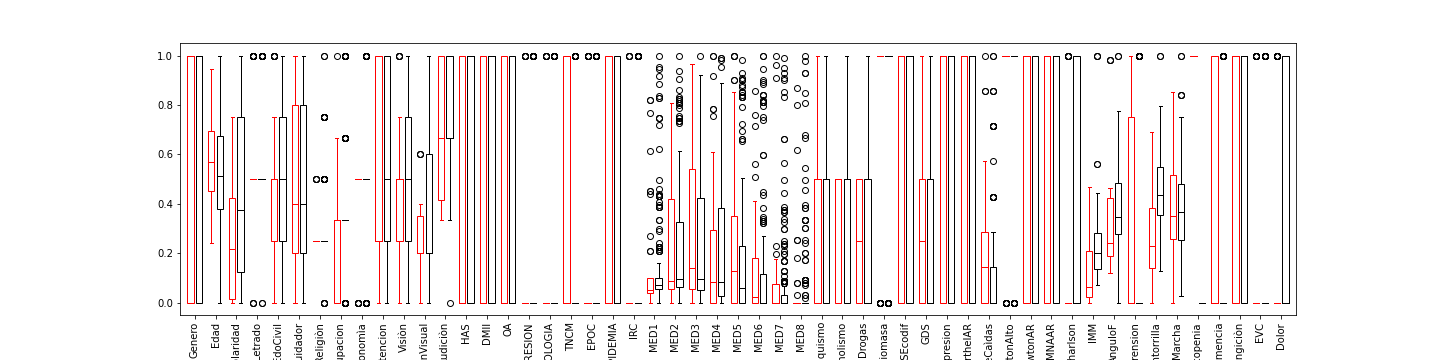
\includegraphics[width=\linewidth]{boxplot_serve_mild.png}
\caption{Boxplot of all remaining features, black boxes are from all mild cases and red from all serve, respectively}
\label{fig:boxplots}
\end{figure*}


\printbibliography[heading=bibintoc, title={References}]
\end{document}
